\documentclass{article}
\usepackage[utf8]{inputenc}
\usepackage{subfig}
\usepackage{amsmath}

\usepackage{graphicx}
\usepackage[a3paper, landscape, margin=0.5cm]{geometry}

\thispagestyle{empty}
% \renewcommand{\thesubfigure}{\roman{subfigure}}
\begin{document}

\begin{figure}[t]
        \centering
        \subfloat[vertical caustics]{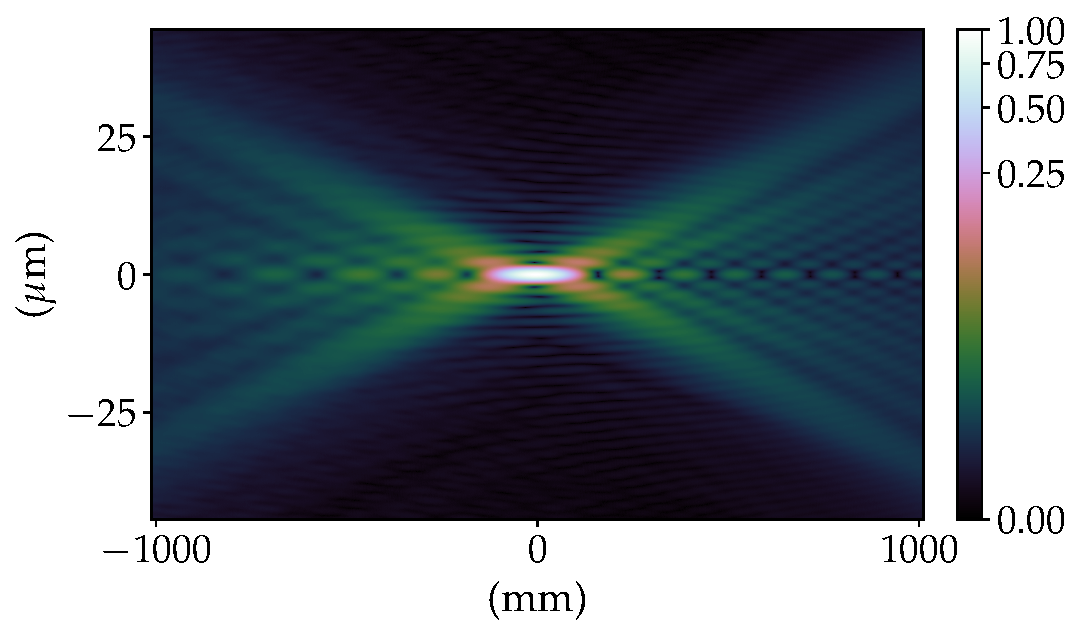
\includegraphics[height=3.4cm]{figures/ch05/CDn01-05-10/Be_CDn_8p0keV_d0p0mm_n1_intensity_cstc_Y_cstc_2D.pdf}}\hspace{0.1cm}
        \subfloat[PSF phase (rad)]{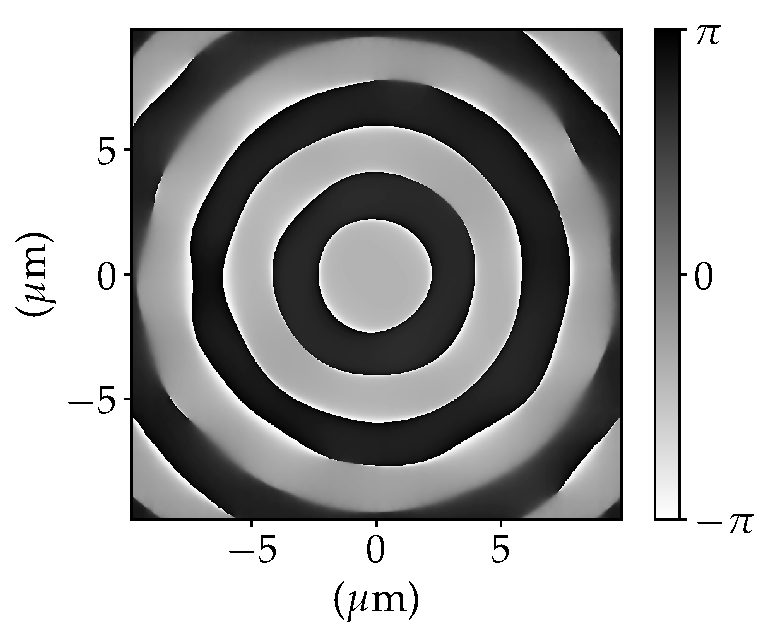
\includegraphics[height=3.5cm]{figures/ch05/CDn01-05-10/Be_CDn_8p0keV_d0p0mm_n1_phase_phase_2D.pdf}}\hspace{0.1cm}
        \subfloat[PSF intensity]{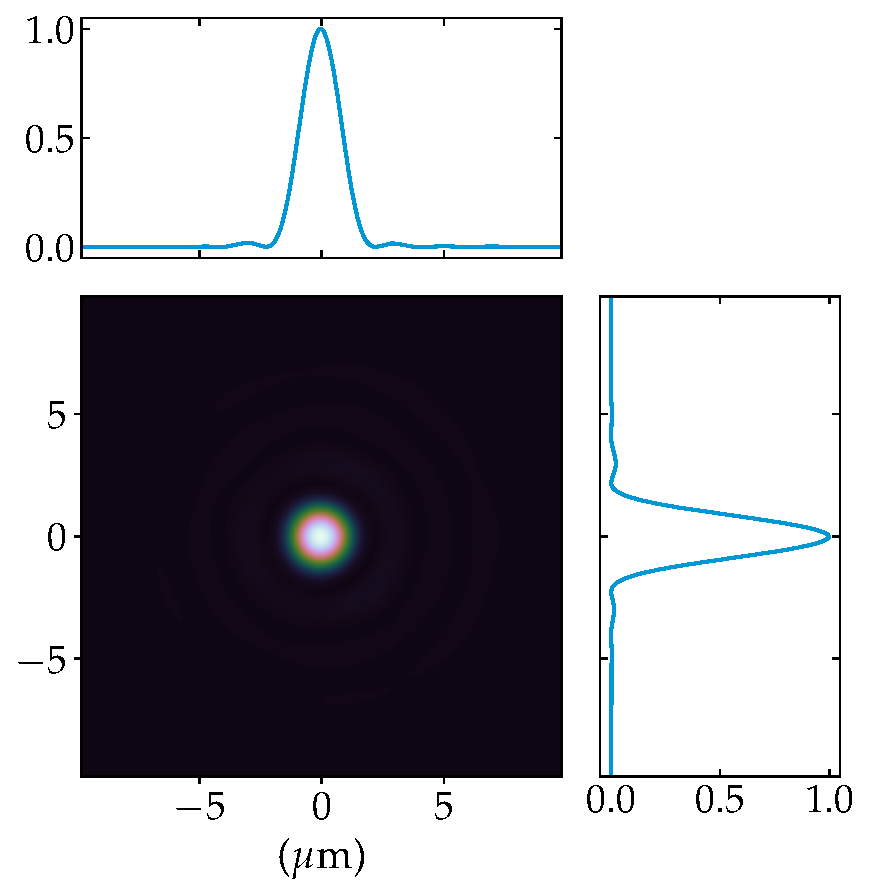
\includegraphics[height=5cm]{figures/ch05/CDn01-05-10/Be_CDn_8p0keV_d0p0mm_n1_intensity_intensity_2D.pdf}}\hspace{0.1cm}
        \subfloat[Strehl ratio]{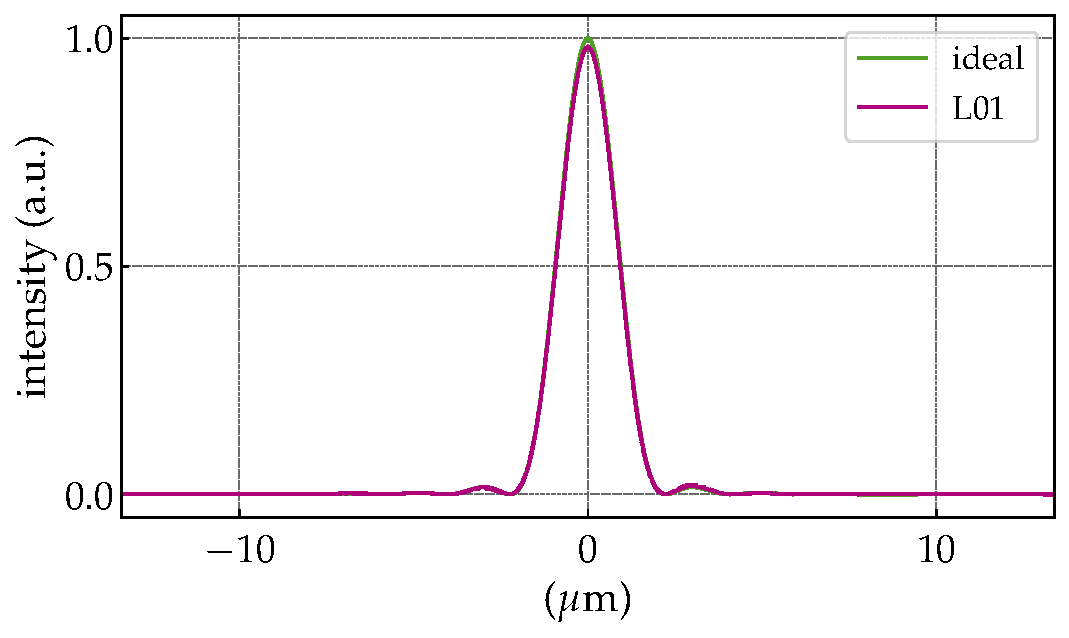
\includegraphics[height=3.45cm]{figures/ch05/CDn01-05-10/L01.pdf}}
        \caption*{L01}\vspace{0.3cm}\setcounter{subfigure}{0}
        \subfloat[vertical caustics]{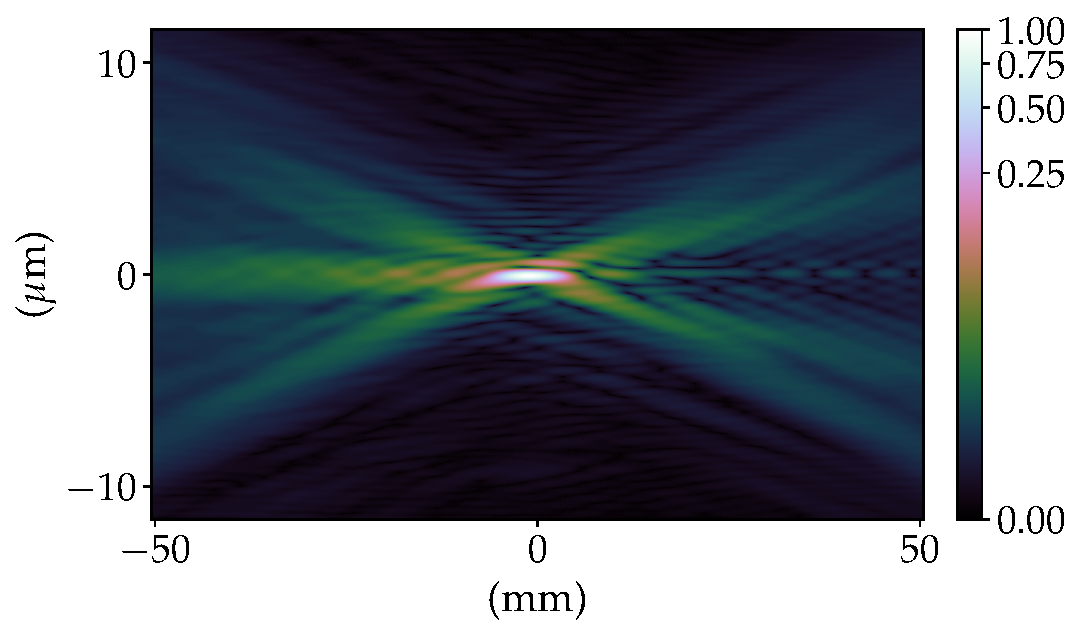
\includegraphics[height=3.4cm]{figures/ch05/CDn01-05-10/Be_CDn_8p0keV_d0p0mm_n5_intensity_cstc_Y_cstc_2D.pdf}}\hspace{0.1cm}
        \subfloat[PSF phase (rad)]{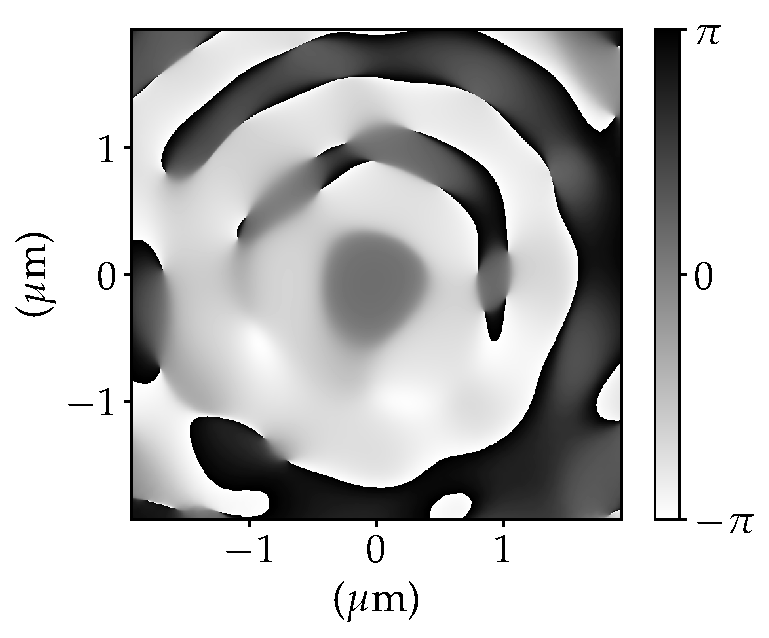
\includegraphics[height=3.5cm]{figures/ch05/CDn01-05-10/Be_CDn_8p0keV_d0p0mm_n5_phase_phase_2D.pdf}}\hspace{0.1cm}
        \subfloat[PSF intensity]{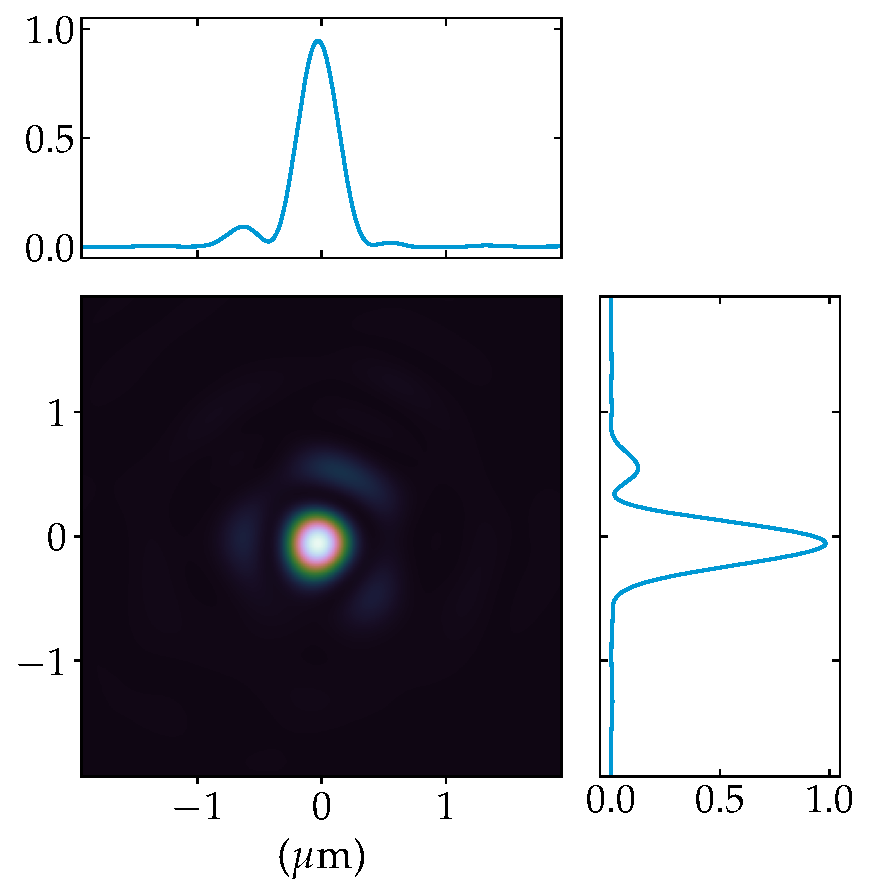
\includegraphics[height=5cm]{figures/ch05/CDn01-05-10/Be_CDn_8p0keV_d0p0mm_n5_intensity_intensity_2D.pdf}}\hspace{0.1cm}
        \subfloat[Strehl ratio]{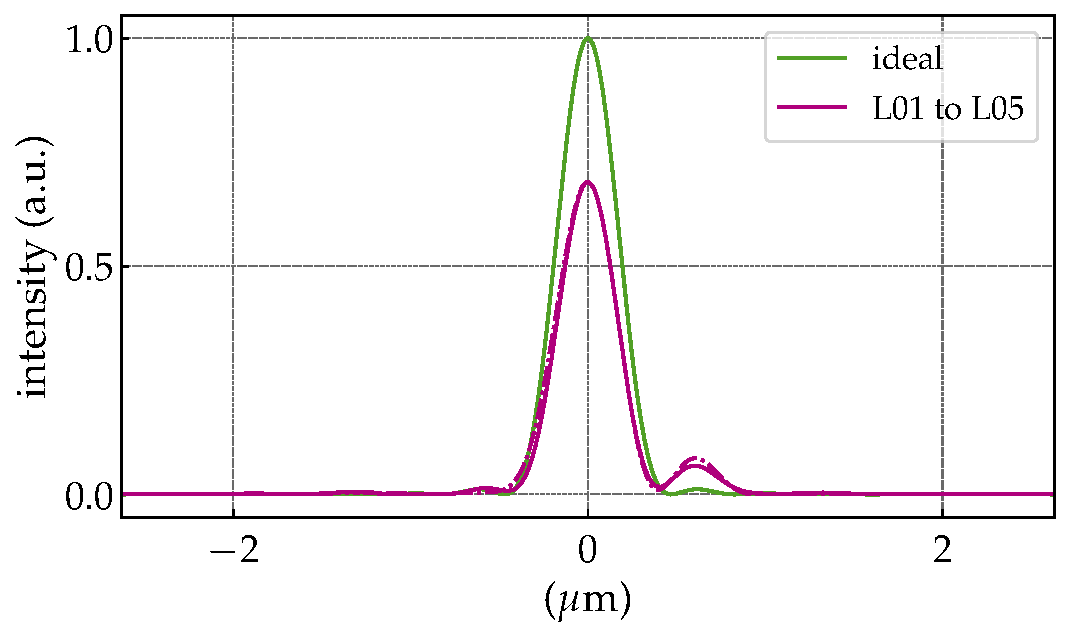
\includegraphics[height=3.45cm]{figures/ch05/CDn01-05-10/L01toL05.pdf}}
        \caption*{L01 to L05 stack}\vspace{0.3cm}\setcounter{subfigure}{0}
        \subfloat[vertical caustics]{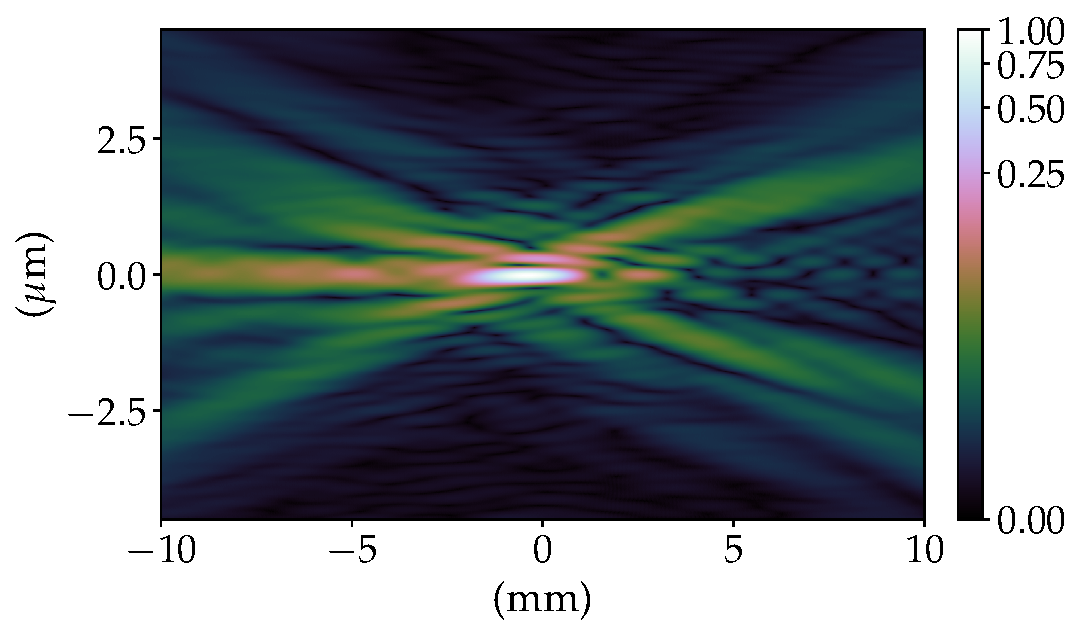
\includegraphics[height=3.4cm]{figures/ch05/CDn01-05-10/Be_CDn_8p0keV_d0p0mm_n10_intensity_cstc_Y_cstc_2D.pdf}}\hspace{0.1cm}
        \subfloat[PSF phase (rad)]{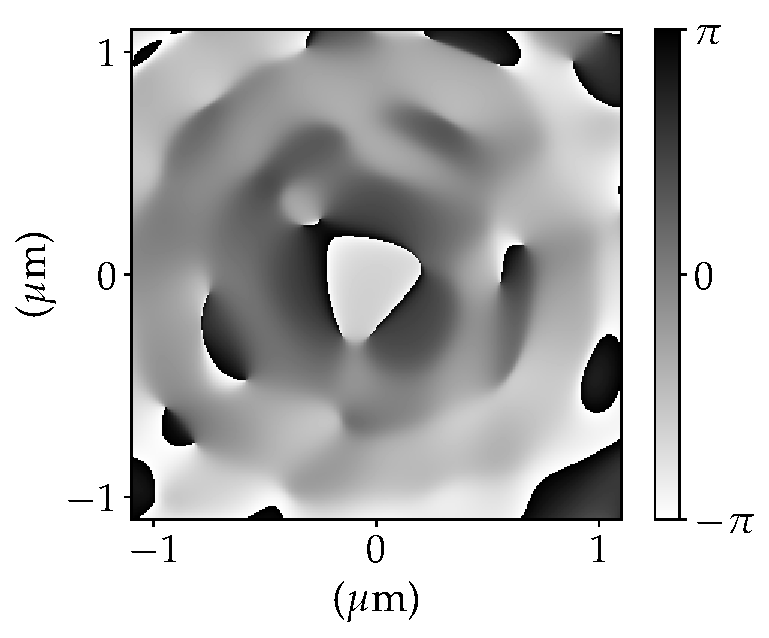
\includegraphics[height=3.5cm]{figures/ch05/CDn01-05-10/Be_CDn_8p0keV_d0p0mm_n10_phase_phase_2D.pdf}}\hspace{0.1cm}
        \subfloat[PSF intensity]{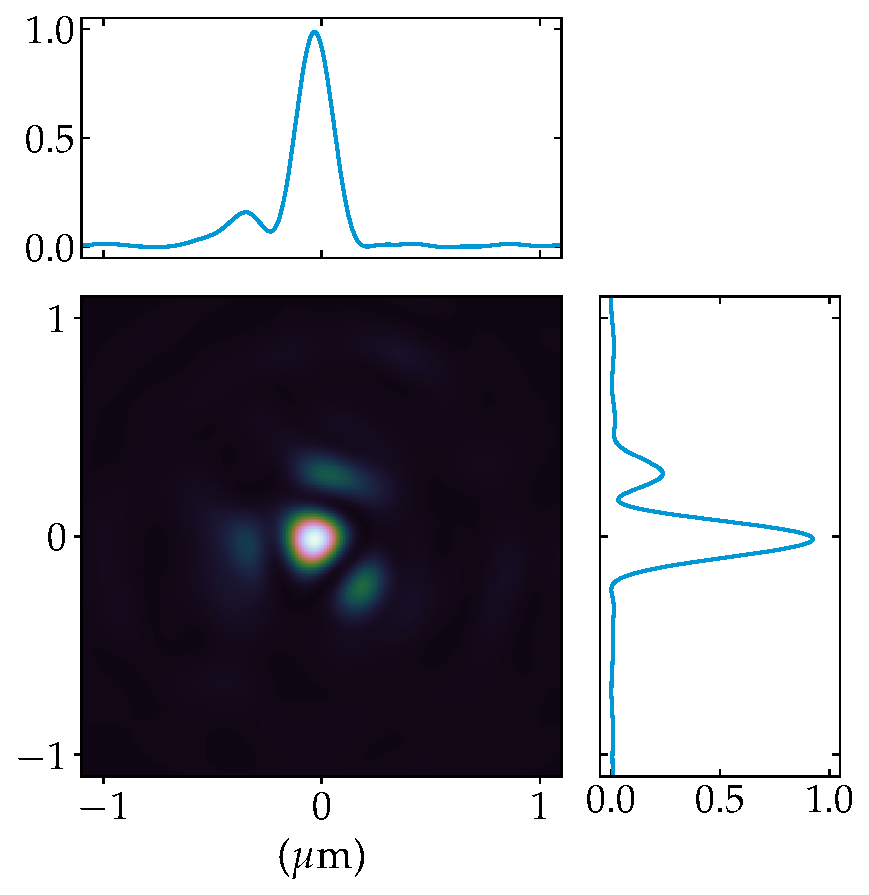
\includegraphics[height=5cm]{figures/ch05/CDn01-05-10/Be_CDn_8p0keV_d0p0mm_n10_intensity_intensity_2D.pdf}}\hspace{0.1cm}
        \subfloat[Strehl ratio]{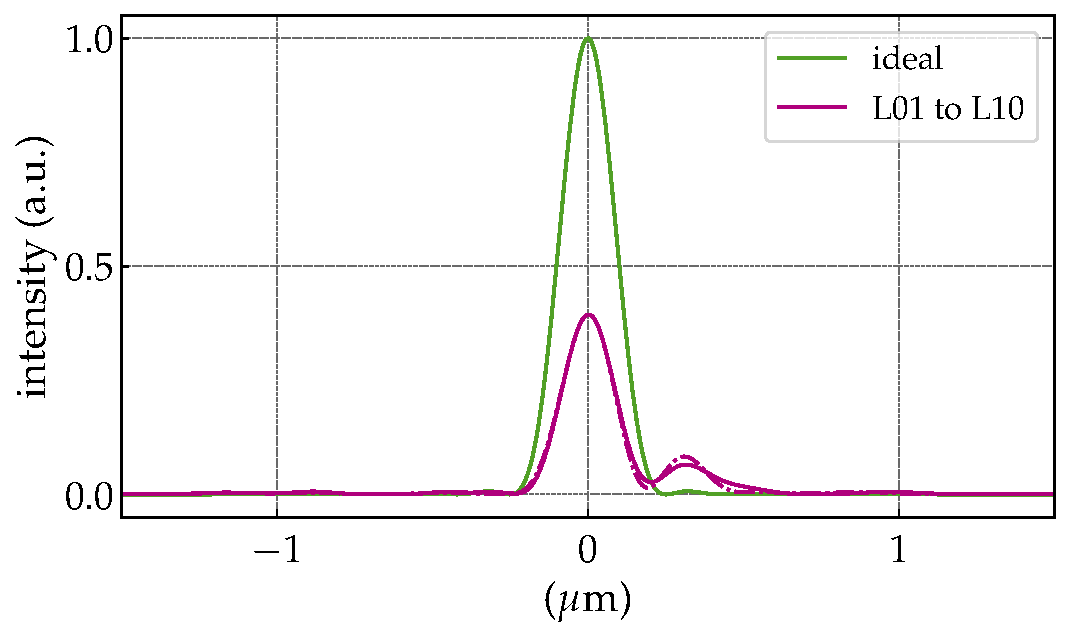
\includegraphics[height=3.45cm]{figures/ch05/CDn01-05-10/L01toL10.pdf}}
        \caption*{L01 to L10 stack}\vspace{0.3cm}
\end{figure}
\end{document}


% \begin{figure}[t]
%         \centering
%         \subfloat[vertical caustics]{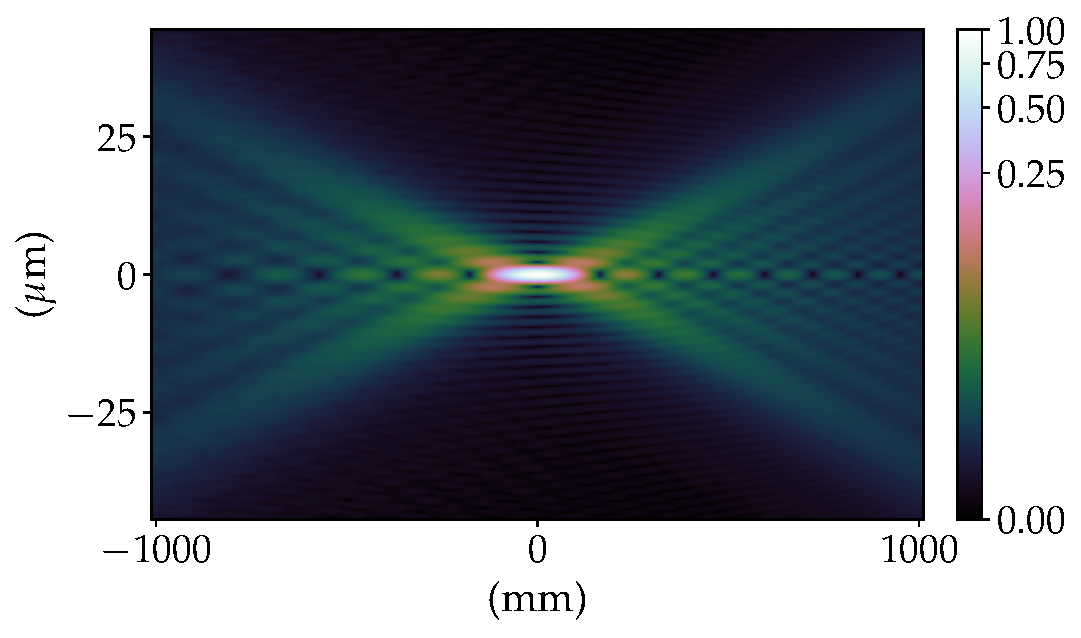
\includegraphics[height=3.4cm]{figures/ch05/CDn01-05-10/Be_ideal_8p0keV_d0p0mm_n1_intensity_cstc_Y_cstc_2D.pdf}}\hspace{0.1cm}
%         \subfloat[PSF phase (rad)]{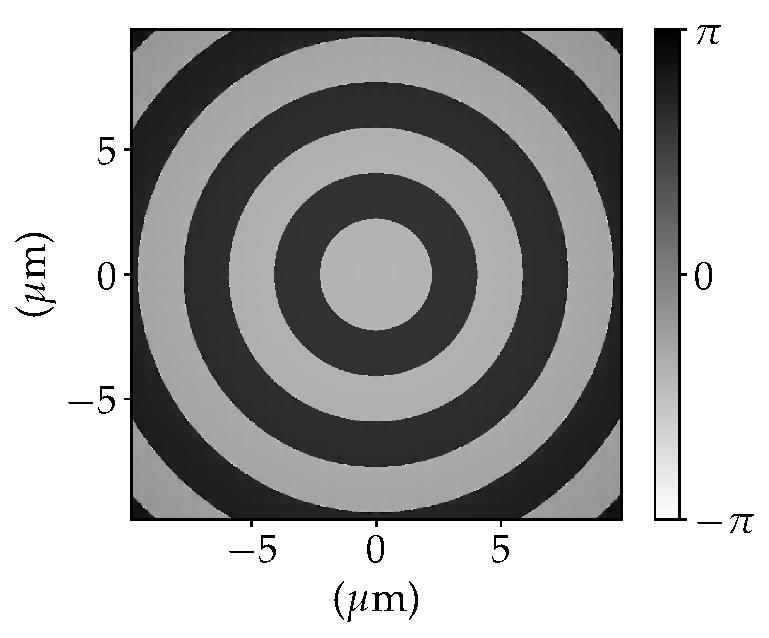
\includegraphics[height=3.5cm]{figures/ch05/CDn01-05-10/Be_ideal_8p0keV_d0p0mm_n1_phase_phase_2D.pdf}}\hspace{0.1cm}
%         \subfloat[PSF intensity]{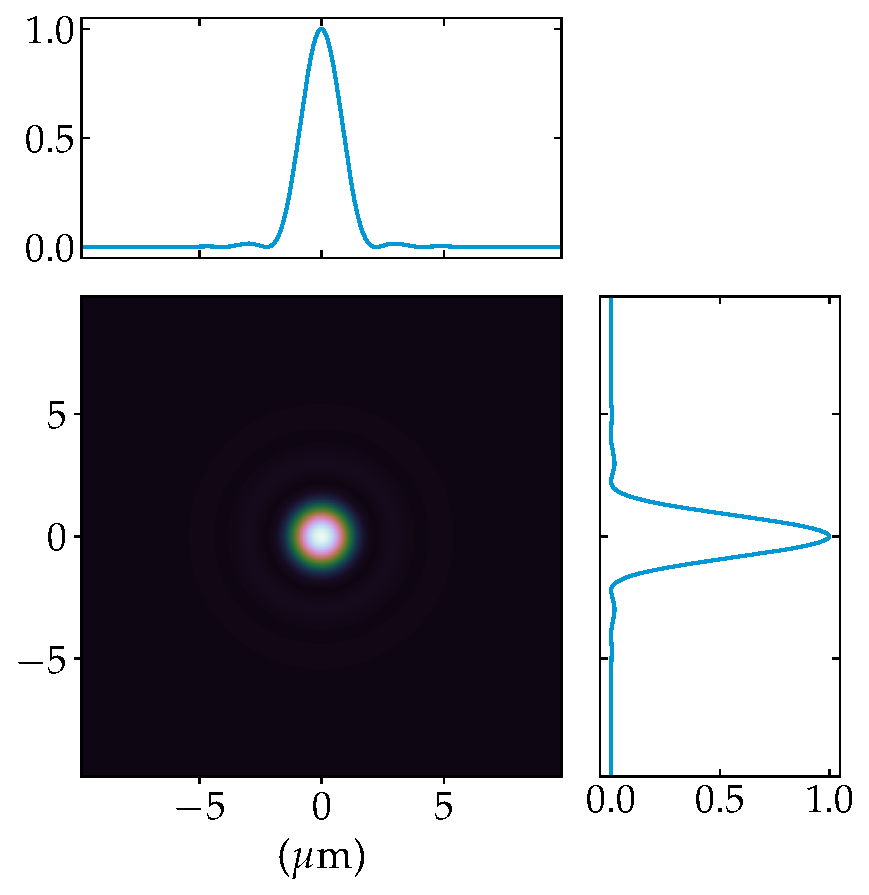
\includegraphics[height=5cm]{figures/ch05/CDn01-05-10/Be_ideal_8p0keV_d0p0mm_n1_intensity_intensity_2D.pdf}}
%         \caption*{L01}\vspace{0.3cm}\setcounter{subfigure}{0}
%         \subfloat[vertical caustics]{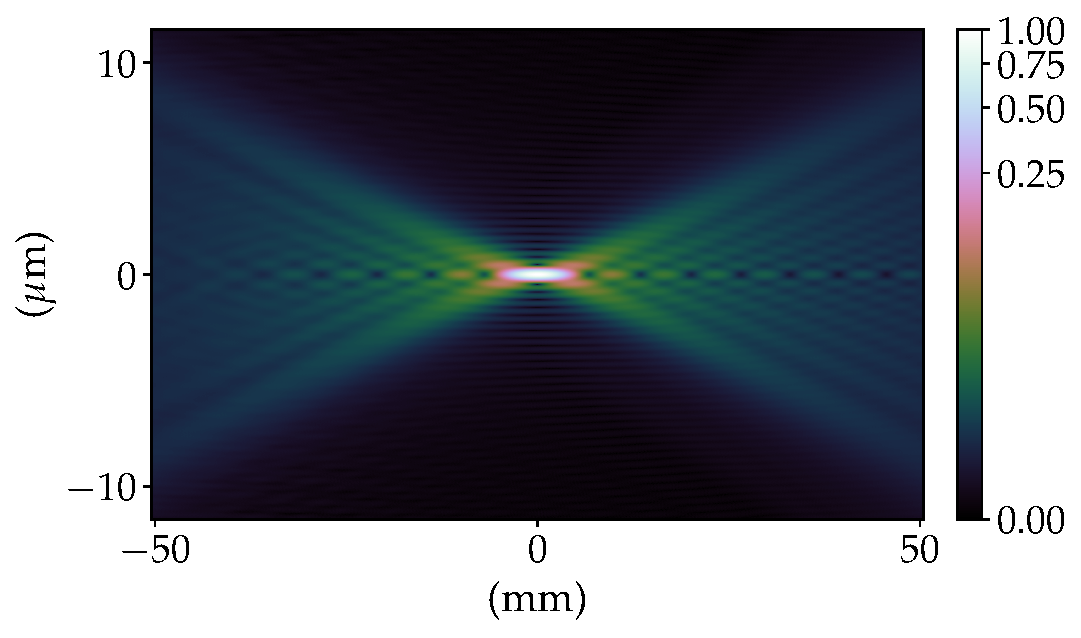
\includegraphics[height=3.4cm]{figures/ch05/CDn01-05-10/Be_ideal_8p0keV_d0p0mm_n5_intensity_cstc_Y_cstc_2D.pdf}}\hspace{0.1cm}
%         \subfloat[PSF phase (rad)]{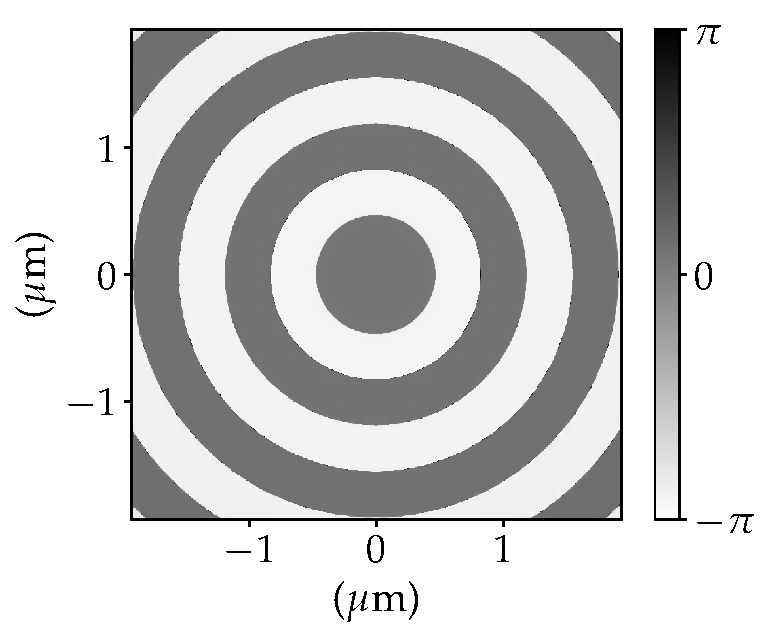
\includegraphics[height=3.5cm]{figures/ch05/CDn01-05-10/Be_ideal_8p0keV_d0p0mm_n5_phase_phase_2D.pdf}}\hspace{0.1cm}
%         \subfloat[PSF intensity]{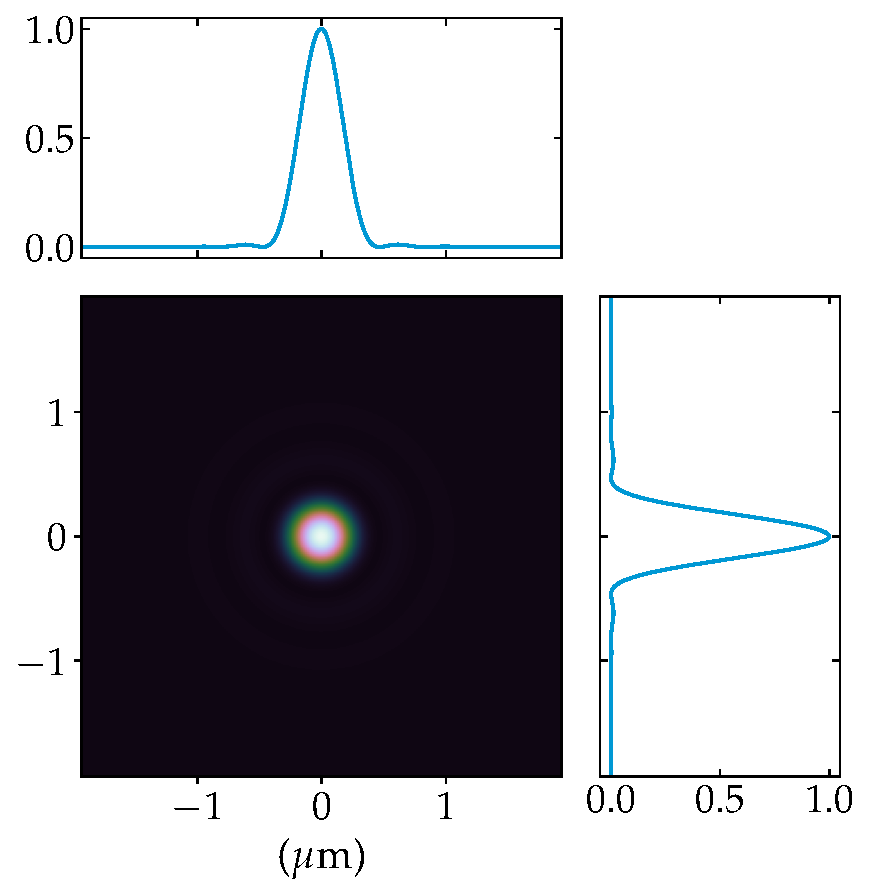
\includegraphics[height=5cm]{figures/ch05/CDn01-05-10/Be_ideal_8p0keV_d0p0mm_n5_intensity_intensity_2D.pdf}}
%         \caption*{L01 to L05 stack}\vspace{0.3cm}\setcounter{subfigure}{0}
%         \subfloat[vertical caustics]{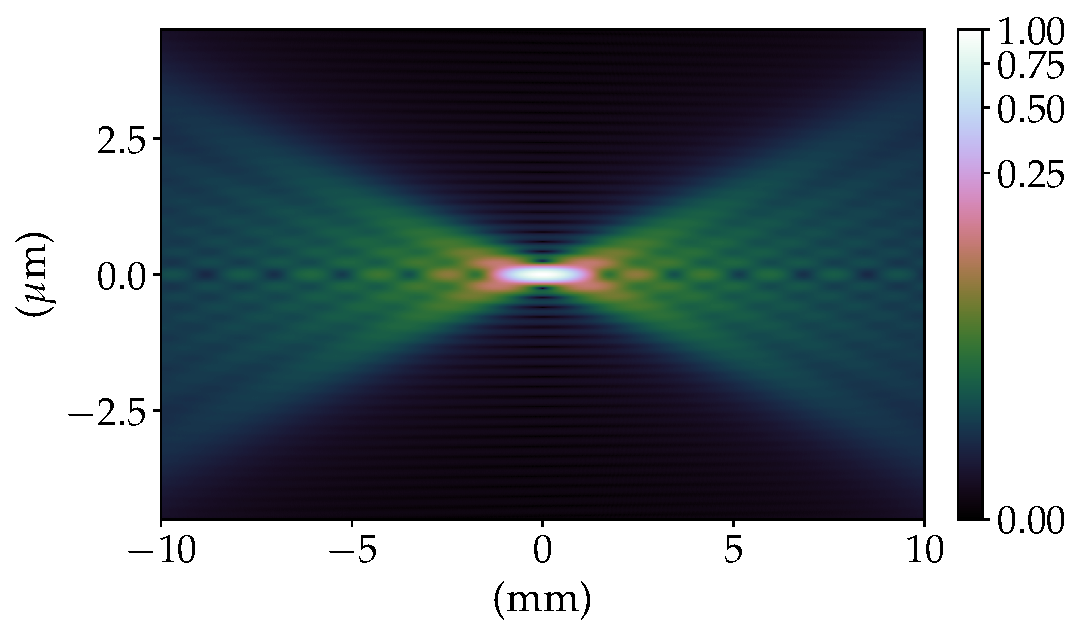
\includegraphics[height=3.4cm]{figures/ch05/CDn01-05-10/Be_ideal_8p0keV_d0p0mm_n10_intensity_cstc_Y_cstc_2D.pdf}}\hspace{0.1cm}
%         \subfloat[PSF phase (rad)]{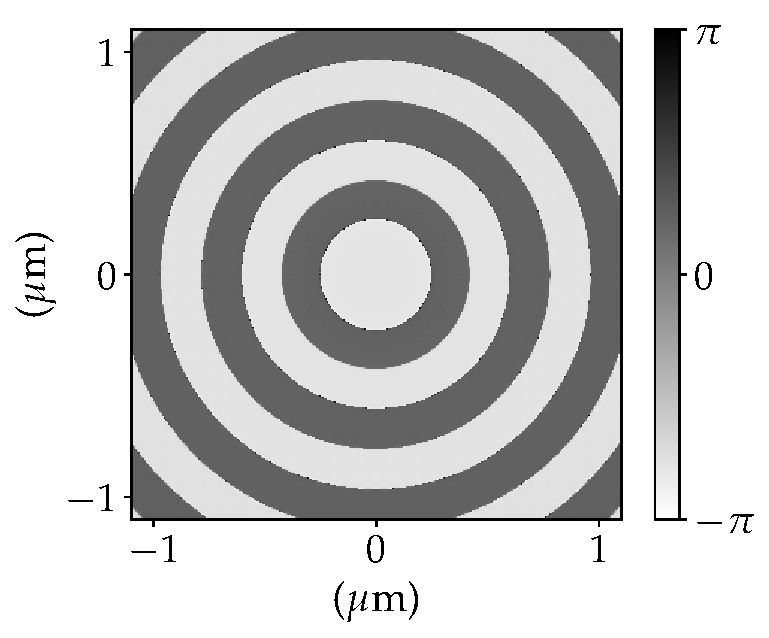
\includegraphics[height=3.5cm]{figures/ch05/CDn01-05-10/Be_ideal_8p0keV_d0p0mm_n10_phase_phase_2D.pdf}}\hspace{0.1cm}
%         \subfloat[PSF intensity]{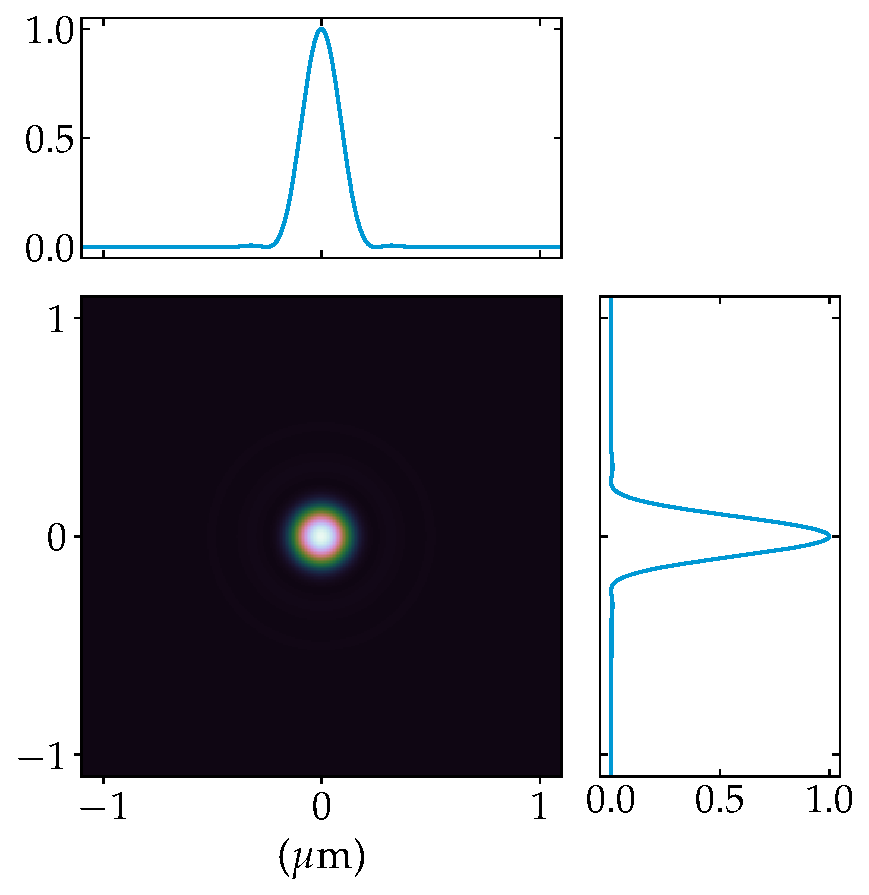
\includegraphics[height=5cm]{figures/ch05/CDn01-05-10/Be_ideal_8p0keV_d0p0mm_n10_intensity_intensity_2D.pdf}}
%         \caption*{L01 to L10 stack}\vspace{0.3cm}\setcounter{subfigure}{0}
% \end{figure}